\documentclass[11pt,a4paper]{article}

\usepackage[margin=2.3cm]{geometry}
\usepackage{lmodern}
\usepackage[T1]{fontenc}
\usepackage{microtype}
\usepackage{amsmath,amssymb}
\usepackage{graphicx}
\usepackage{booktabs}
\usepackage{tabularx}
\usepackage{xcolor}
\usepackage[font=small,labelfont=bf]{caption}
\usepackage{subcaption}
\usepackage[hidelinks]{hyperref}
\usepackage{enumitem}
\setlist{itemsep=2pt,topsep=4pt}

\newcommand{\A}[1]{\alpha_{#1}}
\newcommand{\att}{\rightharpoonup}
\newcommand{\ind}{\hookrightarrow}
\newcommand{\code}[1]{\texttt{#1}}

\title{\textbf{Argumentation Engine}\\[2pt]
\large Abstract Argumentation Semantics and Strategic Argumentation}
\author{Sreenitya Thatikunta}
\date{October 2026}

\begin{document}
\maketitle
\vspace{-1.2em}
\begin{center}
\small Code, tests and data: \url{https://github.com/SreenityaThatikunta/argumentation-engine}
\end{center}

\section{Introduction}

In an argument, some points attack others. Which points should a fair judge
accept? \emph{Abstract argumentation} answers this by modelling a debate as a
directed graph: each node is an argument, and an edge $a \att b$ means
``$a$ attacks $b$''. A \emph{semantics} is a rule for picking the sets of
arguments that can sensibly be accepted together.

This project has two parts, both following Chapter~5 of \emph{Multiagent
Systems} (Rahwan, ``Argumentation among Agents'')~\cite{rahwan}:

\begin{enumerate}
  \item \textbf{An argumentation engine} that computes the standard semantics
        (grounded, complete, preferred, stable and semi-stable), the legal
        in/out/undec labellings, and the acceptance status of each argument.
  \item \textbf{A strategic analysis.} Several agents each hold private
        arguments and choose which to reveal to a judge. The judge accepts the
        grounded extension of everything revealed. We ask \emph{when can an
        agent gain by hiding arguments?} We test two theorems from the book,
        first on random instances and then exhaustively on every small graph.
\end{enumerate}

The main findings are that the book's sufficient condition for
strategyproofness (Theorem~5.4) held in every one of over 200 million cases we
checked, and that the condition is far from necessary. In most strategyproof
cases where it fails, hiding an argument \emph{can} rescue another, but always
at an equal or greater cost.

\section{Background}

An \textbf{argumentation framework} is a pair $\langle A, \att\rangle$ of a
finite set of arguments and an attack relation, as introduced by Dung~\cite{dung}. For a set $S \subseteq A$, let
$S^+$ be the arguments attacked by $S$, and $\alpha^-$ the attackers of
$\alpha$. The book's definitions build on each other:

\begin{itemize}
  \item $S$ is \textbf{conflict-free} if no member attacks another
        ($S \cap S^+ = \emptyset$).
  \item $S$ \textbf{defends} $\alpha$ if it attacks every attacker of $\alpha$
        ($\alpha^- \subseteq S^+$).
  \item The \textbf{characteristic function} $F(S)$ is the set of arguments
        that $S$ defends.
  \item $S$ is \textbf{admissible} if it is conflict-free and
        $S \subseteq F(S)$, and \textbf{complete} if it is conflict-free and
        $S = F(S)$.
\end{itemize}

The semantics then pick out particular complete extensions. \textbf{Grounded}
is the smallest, obtained by applying $F$ to $\emptyset$ until nothing
changes. \textbf{Preferred} extensions are the maximal ones. \textbf{Stable}
extensions attack every argument outside them, and may not exist.
\textbf{Semi-stable} extensions~\cite{caminada} maximise the \emph{range} $S \cup S^+$; they
always exist and coincide with the stable ones whenever those exist.

A \textbf{labelling} marks each argument \emph{in}, \emph{out} or
\emph{undec}. It is legal when an argument is \emph{in} exactly when all its
attackers are \emph{out}, and \emph{out} exactly when some attacker is
\emph{in}. Legal labellings correspond one-to-one with complete extensions.
Finally, an argument is \textbf{skeptically accepted} if it is in every
extension, \textbf{credulously accepted} if it is in at least one, and
\textbf{rejected} otherwise.

\section{The Argumentation Engine}

The engine is a small Python package with no runtime dependencies.

\begin{center}
\small
\begin{tabularx}{\linewidth}{@{}lX@{}}
\toprule
Module & Contents \\
\midrule
\code{framework.py} & framework class: conflict-free, defence, $F(S)$, admissible, complete \\
\code{semantics.py} & grounded, complete, preferred, stable, semi-stable \\
\code{labelling.py}, \code{acceptance.py} & legal labellings; skeptical/credulous/rejected status \\
\code{strategic.py} & mechanism, best responses, Theorem 5.3 and 5.4 checks \\
\code{visualize.py} & Graphviz rendering (used for every figure in this report) \\
\bottomrule
\end{tabularx}
\end{center}

\paragraph{Algorithms.} The grounded extension is computed exactly as
defined, by iterating $F$ from $\emptyset$. To list complete extensions, we
first compute the grounded extension $G$: every complete extension contains
$G$ and excludes $G^+$. The search therefore only branches on the arguments
$G$ leaves undecided, and only along conflict-free sets. Preferred, stable and
semi-stable extensions are then filtered from the complete ones, and each
labelling is built directly from its extension.

\paragraph{Design decisions.}
(1) Frameworks are immutable, so they can be shared and cached safely.
(2) If a semantics has \emph{no} extensions (possible for stable), the book's
Definition~5.8 read literally would call every argument skeptically accepted
but not credulously accepted. We return \emph{rejected} in that case.
(3) Asking about an argument that is not in the framework raises an error
rather than silently returning a wrong answer.

\paragraph{Validation.} The test suite (255 tests, 97\% line coverage of the
library, run in CI on Python 3.10--3.13) is built from the book. On the
book's Figure~5.1 it checks that $F(\emptyset) = \{\A3,\A5\}$,
$F^2(\emptyset) = \{\A1,\A3,\A5\}$, and that $\{\A3,\A5\}$ is admissible but
not complete (Examples~5.5--5.6). On Figure~5.2 it checks the three complete
extensions $\{\A3\}$, $\{\A1,\A3\}$, $\{\A2,\A3\}$ and the two preferred ones
(Examples~5.7--5.8). Beyond the book, complete extensions are compared with a
brute-force check of all $2^n$ subsets on 50 random graphs, and labellings
with all $3^n$ candidate labellings on 30 more. Edge cases include odd
cycles, self-attacks, and a graph where semi-stable picks fewer extensions
than preferred. Figure~5.3 is the one book example not tested, because its
edges appear only in the image.

\section{Strategic Argumentation}

\paragraph{Setting.} This follows the argumentation mechanism design model
of Rahwan, Larson and Tohm\'e~\cite{rlt}, as presented in the book. Each agent $i$ privately holds a set of arguments $A_i$
(its \emph{type}). Agents report a subset of $A_i$: they may hide arguments
but not invent them. The \textbf{grounded direct mechanism} builds the graph
induced by all reported arguments and accepts its grounded extension. An
agent's utility is the number of its own arguments accepted,
$u_i = |o \cap A_i|$. The mechanism is \textbf{strategyproof} if revealing
everything is always a best response, whatever the others report.

\paragraph{Checking Theorem 5.3 (exact test).} Theorem~5.3 says the mechanism
is strategyproof exactly when, for every agent and every combination of
subsets the other agents might reveal, truth-telling maximises utility. We
check this by brute force: for each agent, each combination of the others'
reports, and each subset the agent could reveal. Many profiles reveal the same
union of arguments, so grounded extensions are cached by that union. An
instance with $n$ arguments then needs at most $2^n$ grounded computations
(256 for $n=8$), which makes thousands of instances cheap.

\paragraph{Checking Theorem 5.4 (graph condition).} Write
$\alpha \ind \beta$ if there is an \emph{odd-length} path from $\alpha$ to
$\beta$. Along a chain of attacks, odd steps act as attacks and even steps as
defences, so $\alpha \ind \beta$ means $\alpha$ can work against $\beta$.
Theorem~5.4 says: if no agent holds $\alpha, \beta$ with $\alpha \ind \beta$,
the mechanism is strategyproof. Cycles make ``odd-length path'' ambiguous, so
we implement two readings:
\begin{itemize}
  \item \textbf{Walks} (arguments may repeat). We search over states
        (argument, parity of path length so far). Each state is visited once,
        so cycles cannot cause infinite loops. Going round an odd cycle flips
        the parity, so one pair can be joined both ways.
  \item \textbf{Simple paths} (no repeats). We enumerate paths directly. This
        is exponential, but fast for graphs of this size.
\end{itemize}
Every simple path is a walk, so the walk reading is stricter. In the graph
$g \att u$, $u \att v \att w \att u$, $u \att t$, the only simple path from
$g$ to $t$ has length 2, but the walk $g\,u\,v\,w\,u\,t$ has length 5, so the
readings disagree. Following the theorem's formal statement, we also count
$\alpha = \beta$; a self-attack is the length-1 case, so this enforces the
theorem's requirement that each type be conflict-free.

\paragraph{Examples 5.10 and 5.11.} In Example~5.10, agent $x$ holds
$\{\A1,\A4,\A5\}$, $y$ holds $\{\A2\}$ and $z$ holds $\{\A3\}$, with attacks
$\A1 \att \A2 \att \A3$, $\A3 \att \A4$ and $\A3 \att \A5$. Revealing
everything gives $\{\A1, \A3\}$, so $x$ gets 1. If $x$ hides $\A1$, then
$\A2$ defeats $\A3$, freeing $\A4$ and $\A5$, and $x$ gets 2
(Figure~\ref{fig:ex510}). Our checker finds exactly this deviation, and
Theorem~5.4 flags $\A1 \ind \A4$ and $\A1 \ind \A5$. Example~5.11 adds
$\A6 \in A_x$ with $\A6 \att \A3$. Now $x$ gets all four arguments by telling
the truth: the mechanism is strategyproof even though the condition still
fails.

\begin{figure}[t]
  \centering
  \begin{subfigure}{0.48\linewidth}
    \centering
    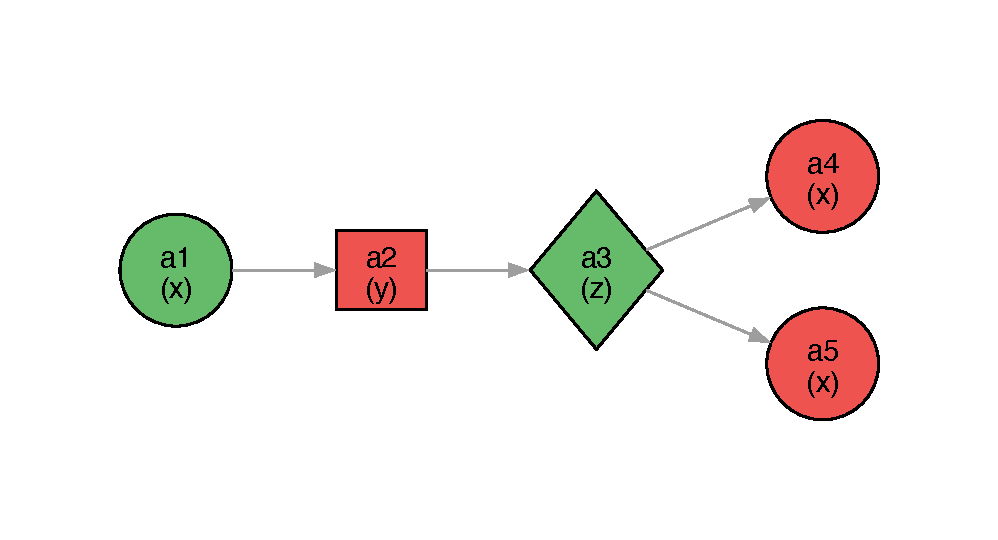
\includegraphics[width=\linewidth]{figures/example_5_10_truthful.pdf}
    \caption{All agents truthful: outcome $\{\A1,\A3\}$, $u_x = 1$.}
  \end{subfigure}\hfill
  \begin{subfigure}{0.48\linewidth}
    \centering
    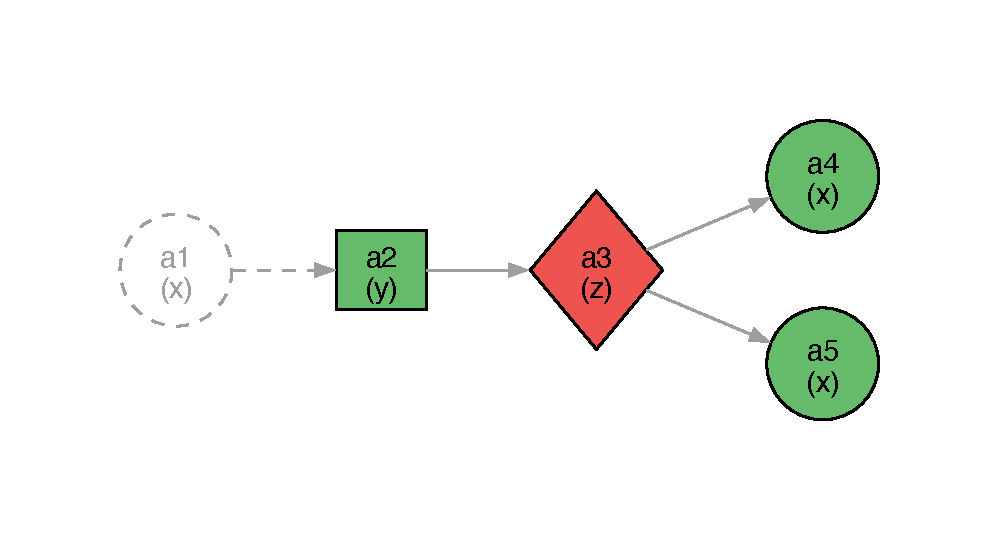
\includegraphics[width=\linewidth]{figures/example_5_10_x_hides_a1.pdf}
    \caption{$x$ hides $\A1$: outcome $\{\A2,\A4,\A5\}$, $u_x = 2$.}
  \end{subfigure}
  \caption{Example 5.10. Green arguments are accepted (in), red are rejected
  (out); the dashed argument is withheld. Each agent has its own node shape.}
  \label{fig:ex510}
\end{figure}

\paragraph{Textbook errata.} We confirmed both known misprints.
(1)~In Example~5.10 the utilities of $y$ and $z$ are written with each other's
argument sets; correctly, $u_y = 0$ (holding $\A2$) and $u_z = 1$ (holding
$\A3$). (2)~After Example~5.11, the argument that cancels the indirect
self-defeat is $\A6$, which attacks $\A3$, not $\A5$.

\section{Experiments}

\paragraph{Setup.} For each $p \in \{0.05, 0.1, 0.15, 0.2, 0.3, 0.4, 0.5\}$
we generated 1000 random instances (7000 in total): 3 agents, 6--8 arguments,
each possible attack $a \att b$ ($a \neq b$) present independently with
probability $p$, and each argument given to a random agent. For every instance
we recorded whether the mechanism is strategyproof (Theorem~5.3) and whether
Theorem~5.4's condition holds under both readings. A second run of 7000
instances also allowed self-attacks. Everything is seeded and reproducible.

\subsection*{Q1: How often is the mechanism strategyproof?}

\begin{table}[h]
\centering
\small
\begin{tabular}{@{}lrrrrrrr@{}}
\toprule
$p$ & 0.05 & 0.10 & 0.15 & 0.20 & 0.30 & 0.40 & 0.50 \\
\midrule
Strategyproof & 95.7\% & 81.2\% & 60.6\% & 44.5\% & 18.1\% & 6.1\% & 3.2\% \\
Theorem 5.4 condition holds & 54.3\% & 22.7\% & 10.9\% & 4.4\% & 0.8\% & 0.1\% & 0.0\% \\
Q2: condition holds, not strategyproof & 0 & 0 & 0 & 0 & 0 & 0 & 0 \\
Q3: strategyproof, condition fails & 414 & 585 & 497 & 401 & 173 & 60 & 32 \\
\bottomrule
\end{tabular}
\caption{Results over 1000 instances per $p$ (no self-attacks).}
\label{tab:q1}
\end{table}

Strategyproofness drops quickly as attacks get denser
(Table~\ref{tab:q1}, Figure~\ref{fig:plot}). With more attacks there are more
chains linking an agent's own arguments, and so more chances for one of them
to work against another. The condition falls even faster, reaching zero at
$p = 0.5$. The walk and simple-path readings gave the same verdict on every
random instance. With self-attacks, strategyproofness is lower at small $p$
(72.7\% vs 81.2\% at $p = 0.1$) but higher at large $p$ (9.5\% vs 3.2\% at
$p = 0.5$). Self-attacking arguments are never accepted, so in dense graphs
almost nothing is accepted at all: on average 0.08 arguments per instance at
$p = 0.5$, against 0.22 without self-attacks. With so little ever accepted,
there is little to gain by hiding.

\begin{figure}[t]
  \centering
  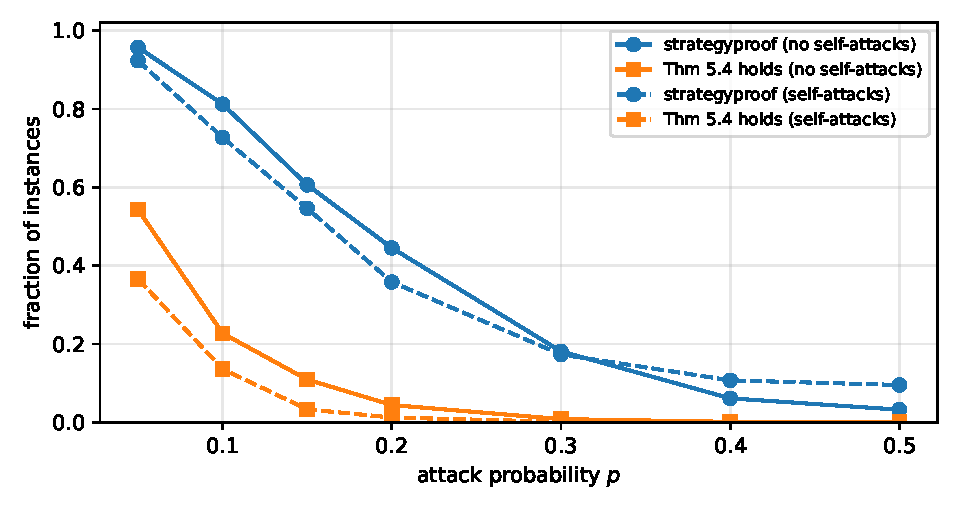
\includegraphics[width=0.78\linewidth]{figures/strategyproofness.pdf}
  \caption{Fraction of instances that are strategyproof (blue) and that
  satisfy Theorem 5.4's condition (orange), without (solid) and with (dashed)
  self-attacks. The gap between the curves is Q3.}
  \label{fig:plot}
\end{figure}

\subsection*{Q2: Does the condition ever hold without strategyproofness?}

\textbf{No.} None of the 14\,000 random instances, with or without
self-attacks, satisfies the condition yet fails strategyproofness, under
either reading. Random sampling can miss rare cases, so we also checked
\emph{exhaustively}. Because agent types do not overlap, the other agents
together can reveal \emph{any} subset of the arguments the agent does not
own. Strategyproofness for one agent therefore depends only on the graph and
the agent's own set, so we checked every directed graph on up to 5 arguments
against every possible own set. A fast bitmask version of the engine,
cross-checked against the main library in the test suite, makes this take
seconds (or about four minutes with self-attacks, which allow $2^{25}$ graphs
at $n = 5$).

\begin{table}[h]
\centering
\small
\begin{tabular}{@{}lrr@{}}
\toprule
Graphs with $n \le 5$ & (graph, own set) pairs & Counterexamples (walks / simple) \\
\midrule
No self-attacks & 6,312,206 & 0 / 0 \\
With self-attacks & 201,656,372 & 0 / 0 \\
\bottomrule
\end{tabular}
\caption{Exhaustive verification of Theorem 5.4.}
\label{tab:exhaustive}
\end{table}

This is what the theorem predicts. Intuitively, if none of an agent's
arguments has an odd path to another of its arguments, then each of them can
only help (defend) the agent's other arguments, never harm them. Revealing
more can therefore never reduce the agent's utility. A notable side result:
the \emph{simple-path} reading never failed either, even though it accepts
more cases than the walk reading (33,549 extra pairs at $n = 5$, all
strategyproof). For graphs of this size, the looser condition is still a valid
test.

\subsection*{Q3: Strategyproof although the condition fails}

\textbf{Yes, very often}: 2162 of the 3094 strategyproof instances (70\%)
fail the condition. This is expected, since the condition is only sufficient.
To see \emph{why} each one is still strategyproof, the experiment script
labels every such instance with one of three reasons:

\begin{center}
\small
\begin{tabularx}{\linewidth}{@{}lrrX@{}}
\toprule
Reason & Count & With self-att. & Meaning \\
\midrule
Rescue costs as much & 2128 (98\%) & 1619 & Hiding can get a rejected own argument accepted, but every such move loses at least as many own arguments. \\
Never rescues & 31 & 447 & Whatever the others reveal, hiding never turns a rejected own argument into an accepted one. \\
Self-cycles only & 3 & 315 & The only violations are $\alpha \ind \alpha$: an odd cycle back to the same argument. \\
\bottomrule
\end{tabularx}
\end{center}

One worked instance of each, taken from the saved results:

\begin{itemize}
  \item \textbf{Rescue costs as much.} Agent $x$ holds $\{\A1,\A2,\A5\}$ and
        the only attack is $\A5 \att \A1$, a direct conflict inside $x$'s own
        set. Telling the truth, $x$ gets $\{\A2,\A5\}$. Hiding $\A5$ rescues
        $\A1$ but loses $\A5$ itself, giving $\{\A1,\A2\}$: still 2. The
        condition only looks at the graph, but utility \emph{counts}
        arguments, so a one-for-one swap is never a strict gain. This is the
        main reason the condition is so conservative.
  \item \textbf{Never rescues.} Agent $y$ holds $\{\A1,\A5\}$, with attacks
        $\A5 \att \A6$, $\A6 \att \A1$, $\A6 \att \A4$ and $\A4 \att \A1$.
        The path $\A5\,\A6\,\A4\,\A1$ has length 3, so $\A5 \ind \A1$. But
        $\A5$ also \emph{defends} $\A1$ through the length-2 path
        $\A5\,\A6\,\A1$. Whenever the harmful route is active, the helpful
        one is too, so hiding $\A5$ never gets $\A1$ accepted. This is the
        same effect that $\A6$ has in Example~5.11.
  \item \textbf{Self-cycles only.} With $\A1 \att \A2 \att \A6 \att \A1$
        (plus $\A2 \att \A1$), each of $\A1$, $\A2$, $\A6$ lies on a 3-cycle
        and so has an odd path to itself. All three belong to different
        agents, and hiding your own argument from a cycle cannot make that
        same argument accepted. The violation is harmless. Self-attacks make
        this case much more common (315 instances).
\end{itemize}

\section{Limitations and Conclusion}

The exhaustive check stops at 5 arguments; $n = 6$ has $2^{30}$ graphs and
would need symmetry reduction to be practical. The single-agent reduction
relies on agent types not overlapping, as in our experiments; the book allows
overlap. Brute-force checking is exponential, which is fine for 6--8
arguments but not for large debates. Figure~5.3 remains untested.

In summary, we built and tested a complete argumentation engine, implemented
the grounded direct mechanism with an exact strategyproofness check, and
studied Theorem~5.4 both statistically and exhaustively. The theorem held in
every case, including under the looser simple-path reading. Its condition is
very conservative, however: in most strategyproof cases where it fails,
hiding an argument could rescue another but never at a profit, because the
condition ignores that the agent is \emph{counting} its accepted arguments.

\begin{thebibliography}{9}\small
\bibitem{rahwan} I.~Rahwan. Argumentation among agents. In G.~Weiss (ed.),
  \emph{Multiagent Systems}, 2nd ed., Chapter 5. MIT Press, 2013.
\bibitem{dung} P.~M.~Dung. On the acceptability of arguments and its
  fundamental role in nonmonotonic reasoning, logic programming and n-person
  games. \emph{Artificial Intelligence}, 77(2):321--357, 1995.
\bibitem{caminada} M.~Caminada. Semi-stable semantics. In \emph{Proc.\
  COMMA 2006}, pages 121--130. IOS Press, 2006.
\bibitem{rlt} I.~Rahwan, K.~Larson and F.~Tohm\'e. A characterisation of
  strategy-proofness for grounded argumentation semantics. In \emph{Proc.\
  IJCAI 2009}, pages 251--256, 2009.
\end{thebibliography}

\end{document}
